\section{Numerical Results}
In this section, the novel scheme is validated against analytical solutions and compared with other schemes.

\subsection{Dam Break on a Wet Domain without Friction}\label{DBwet}
This benchmark is a classical Riemann problem which can be represented by a dam separating two basins with different water depths. The dam is instantaneously removed and the flow patterns are simulated. The analytical solution was firstly introduced in \cite{stoker}. Simple overview of this solution can be also found in \cite{swashe}. The initial conditions of the water depth within our simulation are 
\begin{equation}
h(x)=\begin{cases}
h_l, \text{ for } 0<x<x_0\\
h_r, \text{ for } x_0<x<L\\
\end{cases}
\end{equation}
where $h_l=5$ m, $h_r=3$ m, the position of the dam is $x_0=5$ m and the length of the computational domain is $L=10$ m. The computation is stopped at the time $t=0.5$ s and compared with the DGFEM global limiting scheme (DGFEM GL) where the minmod limiter was used for the shock detection. The solution of the water level can be seen in Figure \ref{shock}. This figure shows the results computed by ten finite elements. 
\begin{figure}
\centering
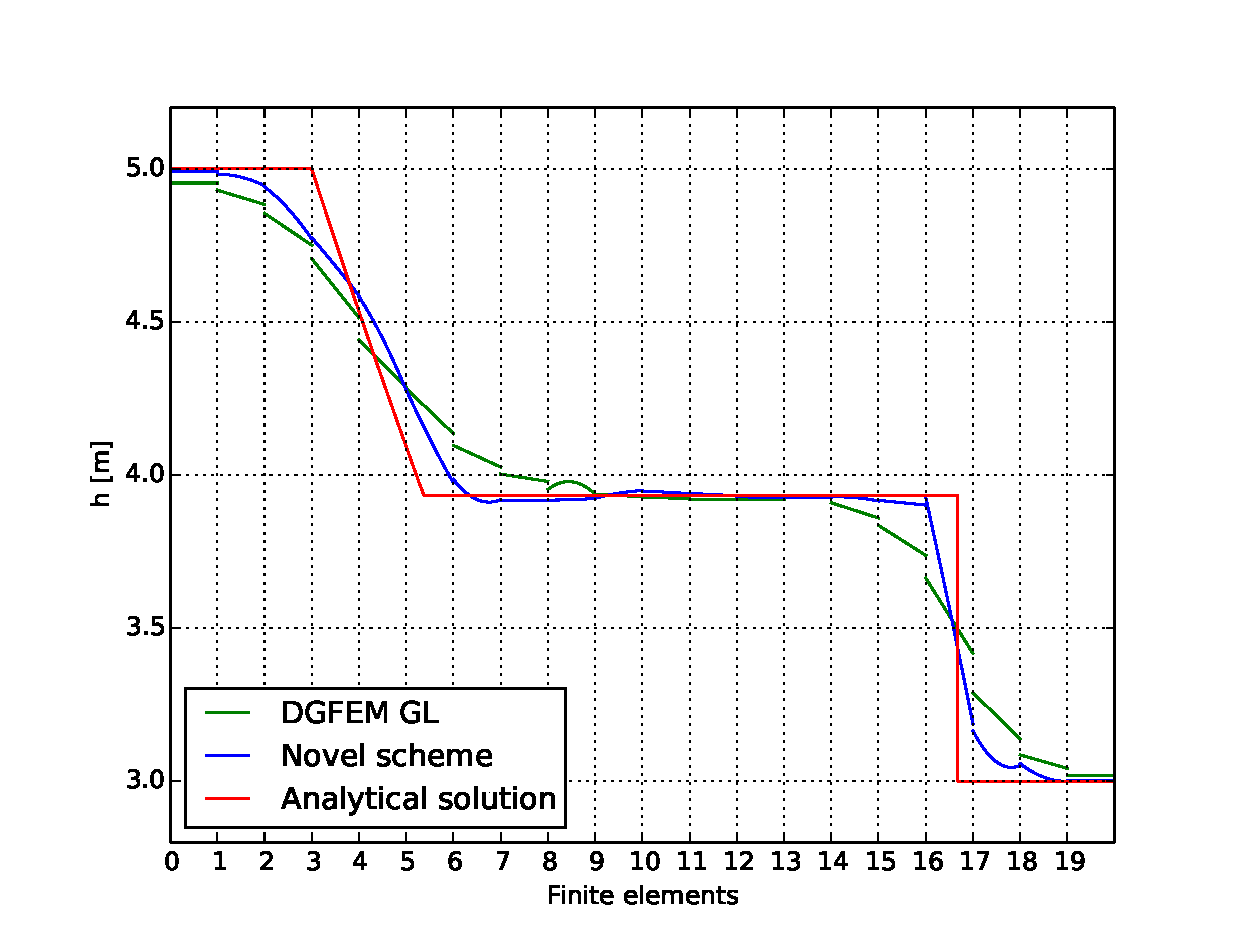
\includegraphics[width=0.7\textwidth]{OBR/shock.eps}
\caption{Simulation of the water level. Comparison of the global limiting and novel scheme.}\label{shock}
\end{figure}
The convergence of a scheme for given test case can be found by the slope of the $log(L_2 \text{error})$ dependent on $log(n_t)$. This slope can bee seen in Figure \ref{L2}. $L_2$ error was computed as
\begin{equation}\label{L2er}
L_2 \text{ error}=\sqrt{\frac{\sum_{i=1}^{n_t} (h_n(x_i)-h_a(x_i))^2 \Delta x_i}{L} }
\end{equation}
where $x_i$ are middle points of the finite elements, $\Delta x_i$ is cell width and $h_{n}$/$h_a$  means the numerical/analytical solution. The slopes of the convergence in Figure \ref{L2} were computed by the linear regression of $L_2$ errors. Numerical results shown that the novel scheme gives better accuracy and convergence of the DGFEM.
\begin{figure}
\centering
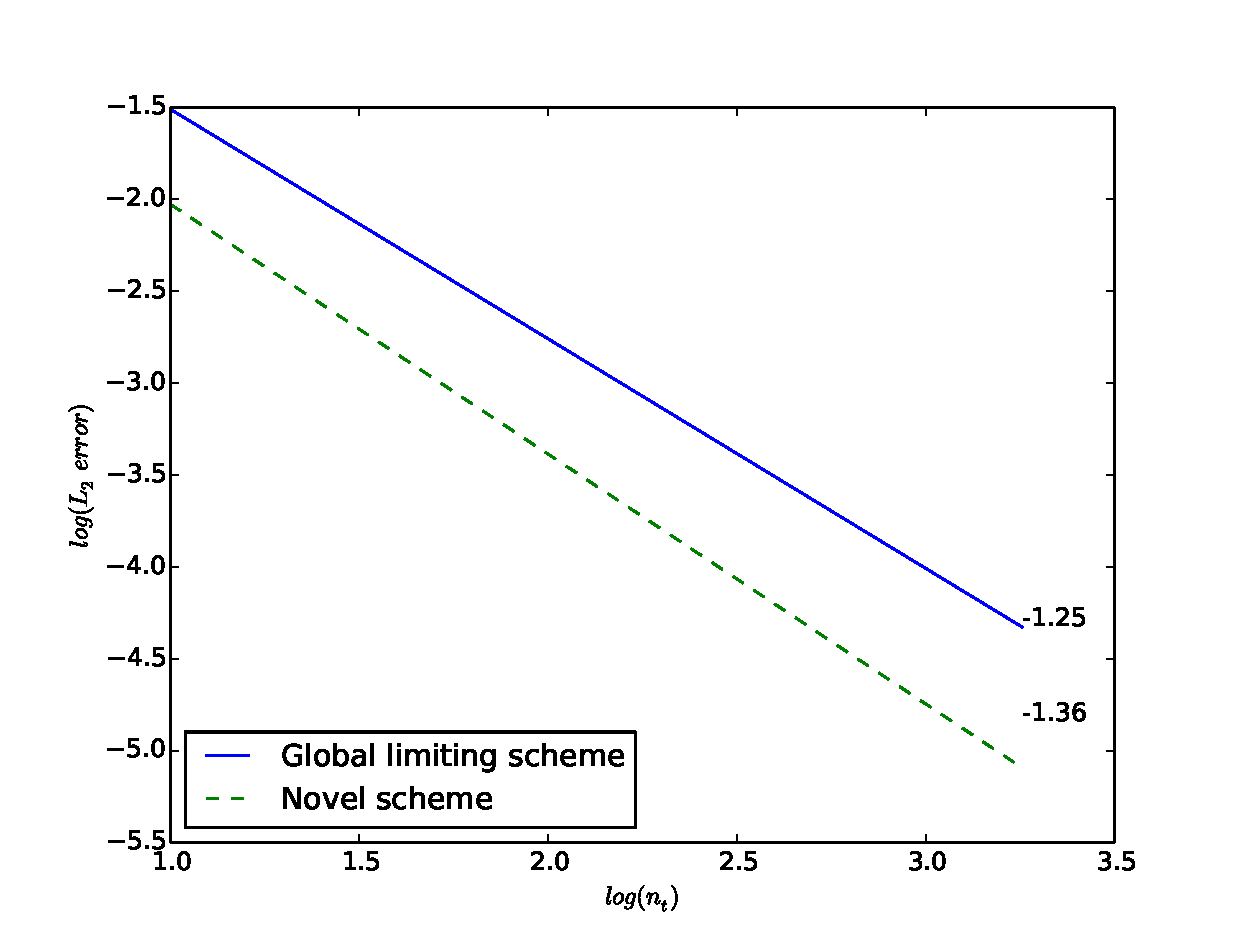
\includegraphics[width=0.7\textwidth]{OBR/shockConverg.eps}
\caption{$L_2$ error convergence of the global limiting and novel scheme.}\label{L2}
\end{figure}


\subsection{Planar surface flow in a parabola}\label{psp}
Another benchmark is the planar surface in a parabola without friction. In this bench mark the the wetting and drying processes occur. Two-dimensional exact solution was derived in \cite{Thacker2006}. 
Here, one-dimensional simplification presented in \cite{swashe} is computed. 
The topography is a parabolic shape given by 
\begin{equation}
B(x)=h_0 \left( \frac{1}{a^2}\left(x-\frac{\text{L}}{2}
\right)^2-1\right).
\end{equation}
The analytical solution of the water depth is
\begin{equation}\label{initPar}
h(x)=\begin{cases}
-h_0 \left(\left(\frac{1}{a}\left(x-\frac{\text{L}}{2}\right)
+\frac{C}{\sqrt{2gh_0}}\cos\left(\frac{\sqrt{2gh_0}}
{a}t\right)\right)^2-1\right) \quad \text{for} 
\ x_1(t)\leq x\leq x_2(t),\\
0 \quad \text{otherwise},
\end{cases}
\end{equation}
with location of the wet/dry interfaces at time $t$ being calculated as
\begin{equation}
\begin{array}{c}
x_1(t)=-\frac12\cos\left(\frac{\sqrt{2gh_0}}{a}t\right)
-a+\frac{\text{L}}{2},\\
x_2(t)=-\frac12\cos\left(\frac{\sqrt{2gh_0}}{a}t\right)
+a+\frac{\text{L}}{2}
\end{array}
\end{equation}
and 
\begin{equation}
C=\sqrt{\frac{2gh_0}{2a}}.
\end{equation}
Initial conditions of the water depth are given by (\ref{initPar}) for $t=0$~s and the flow velocity is zero.

 In the simulation the following parameters were used: $a=1$ m, $h_0=0.5$ m and $L=4$ m. Comparison of the simulations and analytical solution was done in time  $T=5\frac{a\pi}{\sqrt{2gh_0}}$. For the comparison $L_2$ error (\ref{L2er}) was used. Novel scheme is compared by the second order accurate DGFEM scheme. Within second order accurate scheme, the solution is described by the linear function, thus minmod limiter and global limiting method was used for the limiting of the solution. Moreover the scheme was compared with the finite volume scheme with linear reconstruction presented in \cite{fiser2016}. Visual comparison with the exact solution, for different numbers of finite elements/volumes, can be seen in Figures \ref{10}, \ref{20}, \ref{30} and \ref{40}.  WHICH REFERENCE SCHEMES WERE USED? !!!!!!!!!!!!!!!!!!!!!!!
				\begin{figure}[!ht]
								\centering
								 \begin{minipage}[t]{0.44\textwidth}
								    \begin{center}
								    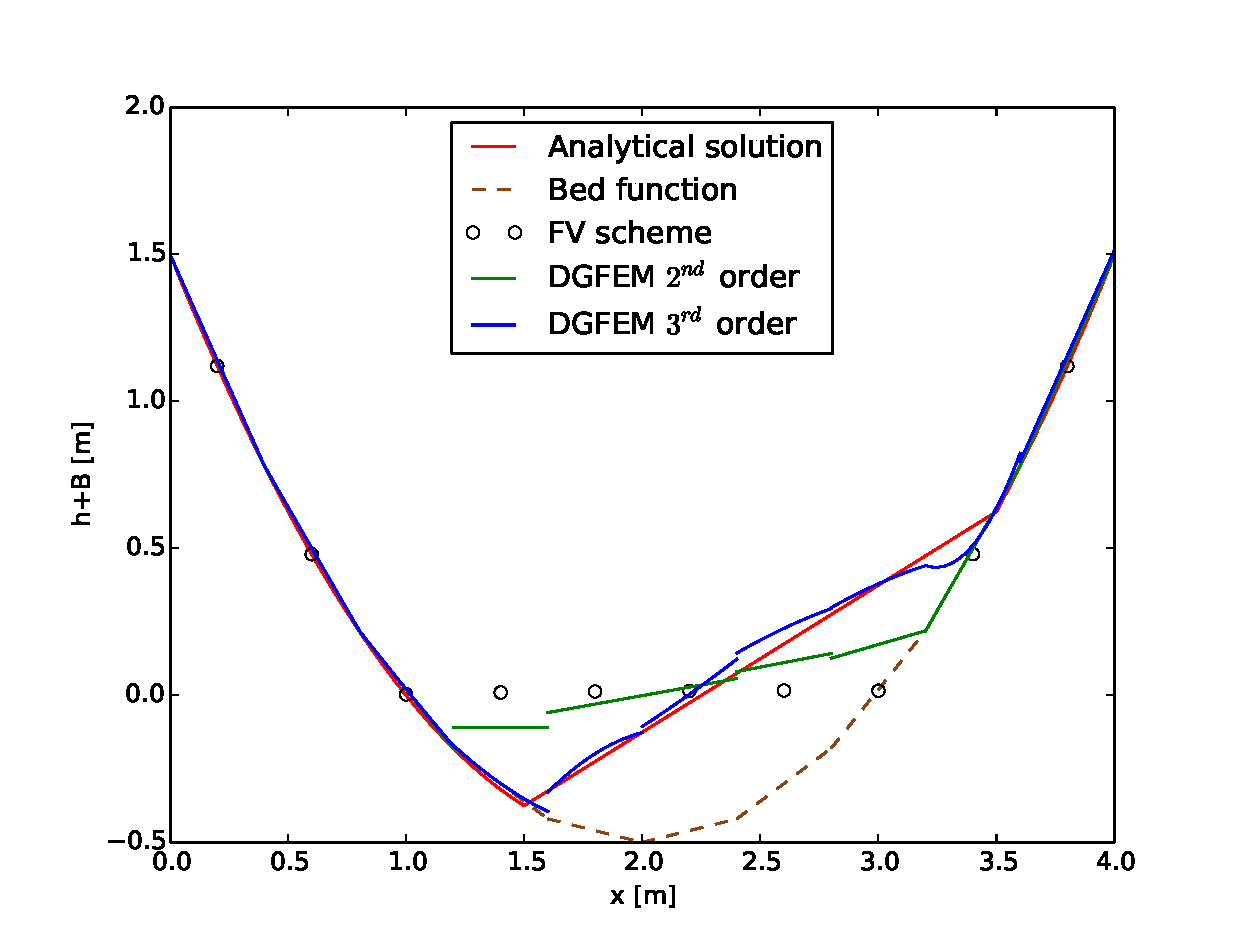
\includegraphics[width=1.0\textwidth]{OBR/10.eps}
								    \caption{Analytical solution compared with the novel and reference scheme-10 finite elements/volumes.}\label{10}
								    \end{center}
								\end{minipage}\hspace{15mm}
								\begin{minipage}[t]{0.44\textwidth}
								    \begin{center}
								    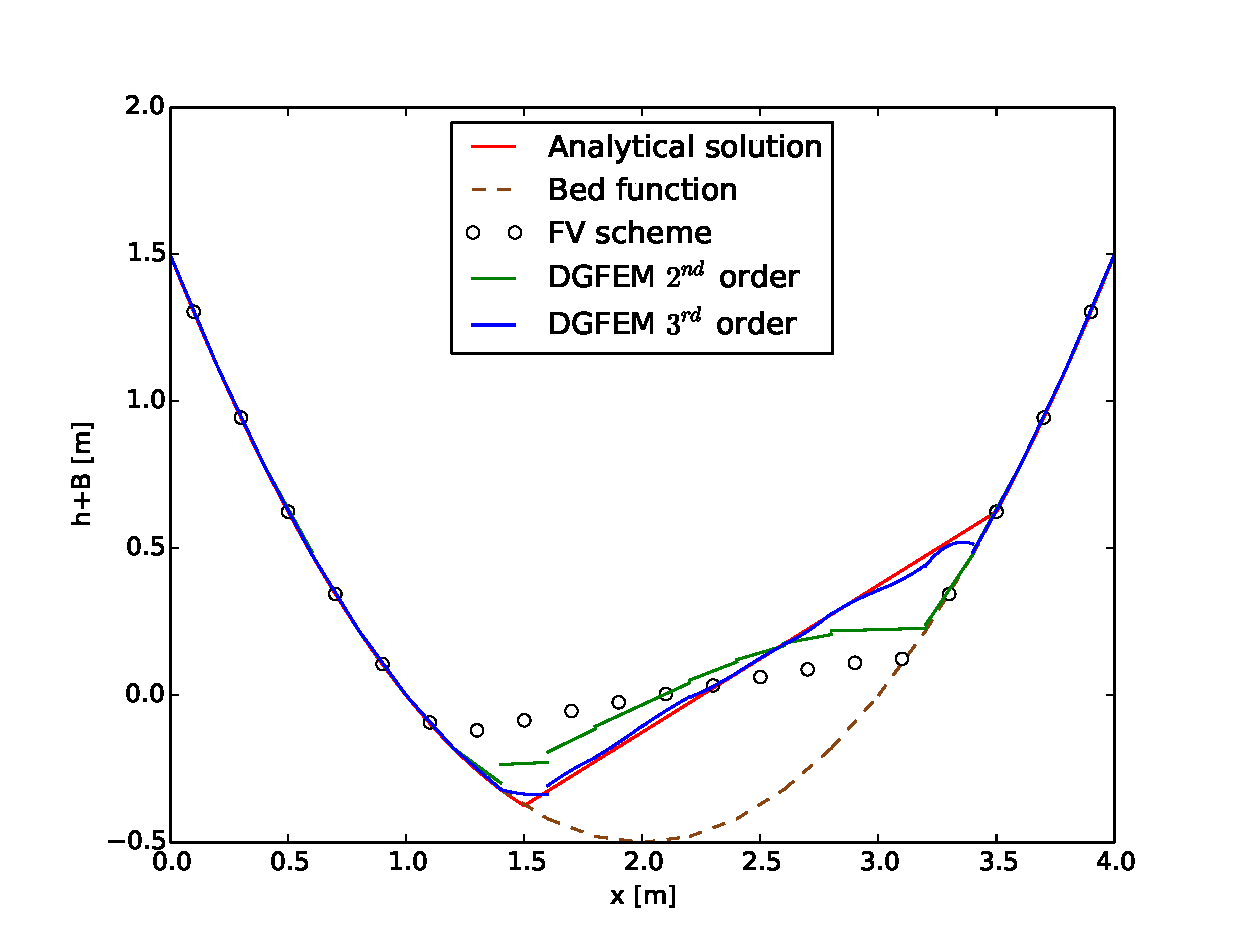
\includegraphics[width=1.0\textwidth]{OBR/20.eps}
								    \caption{Analytical solution compared with the novel and reference scheme-20 finite elements/volumes.}\label{20}
								    \end{center}
								\end{minipage}
				\end{figure}
\begin{figure}[!ht]
								\centering
								 \begin{minipage}[t]{0.44\textwidth}
								    \begin{center}
								    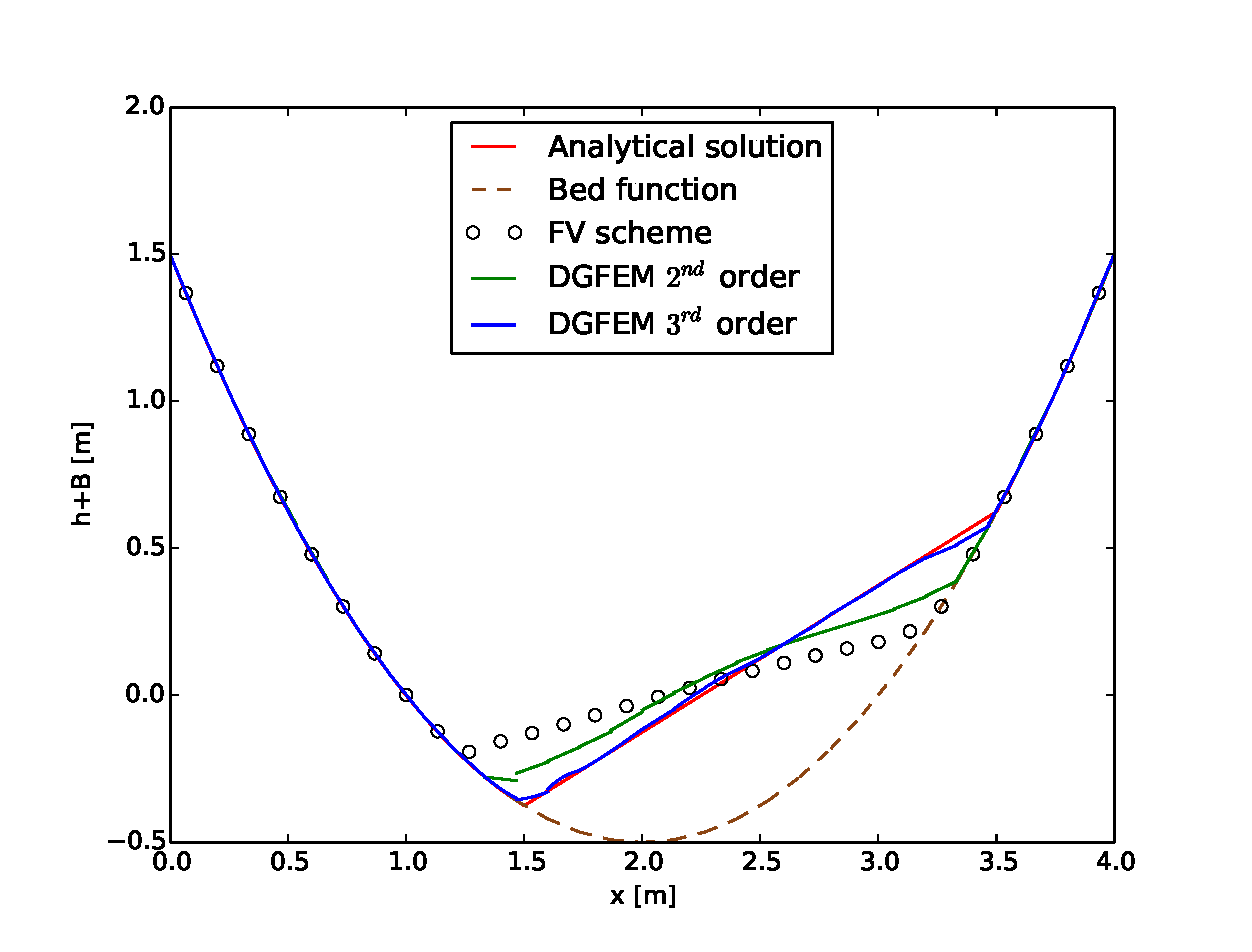
\includegraphics[width=1.0\textwidth]{OBR/30.eps}
								    \caption{Analytical solution compared with the novel and reference scheme-30 finite elements/volumes.}\label{30}
								    \end{center}
								\end{minipage}\hspace{15mm}
								\begin{minipage}[t]{0.44\textwidth}
								    \begin{center}
								    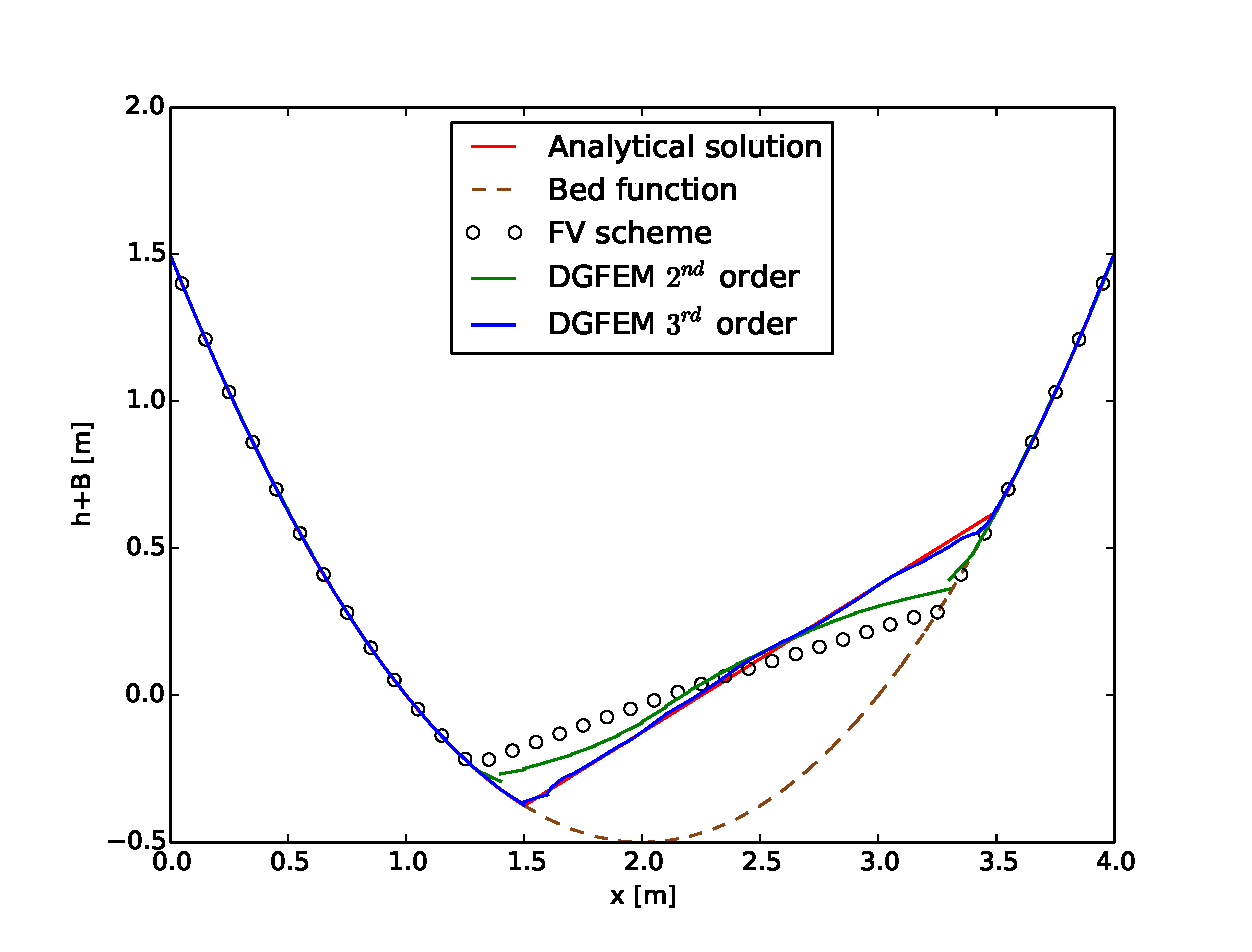
\includegraphics[width=1.0\textwidth]{OBR/40.eps}
								    \caption{Analytical solution compared with the novel and reference scheme-40 finite elements/volumes.}\label{40}
								    \end{center}
								\end{minipage}
				\end{figure}
$L_2$ error convergence is shown in Figure \ref{ParL2}.
\begin{figure}
\centering
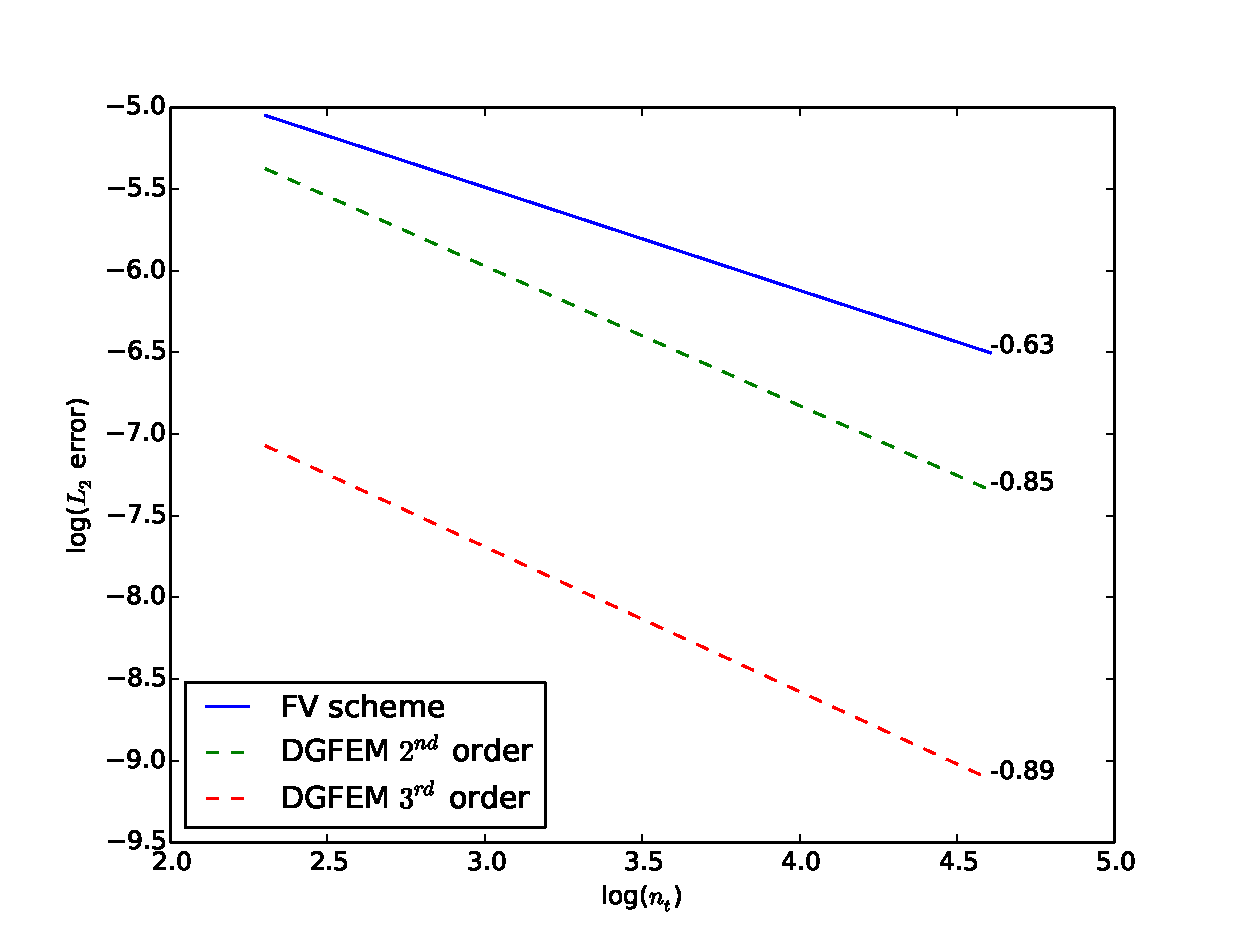
\includegraphics[width=0.7\textwidth]{OBR/ParL2.eps}
\caption{$L_2$ error convergence of the reference FV scheme and novel DGFEM scheme.}\label{ParL2}
\end{figure}

\subsection{Flow over the Bump}
 Another testing benchmark is steady state flow over the bump. The length of the computational domain is L=25 m with a topography given by
\begin{equation}
B(x)=\begin{cases}
 0.2-0.05(x-10)^2  & \text{if 8 m} < x < \text{12 m},\\
0  & \text{else.}
\end{cases}
\end{equation}
In the following, the numerical results of subcritical flow, transcritical flow and transcritical flow with the shock are shown. The results were computed for coarse mesh created by 20 finite elements. The inlet is set on the left side of the computational domain and the outlet is set on the right side of the computational domain. Initial conditions for all these three types of flow are 
\begin{equation}
\begin{array}{ccc}
h(x)+B(x)=2,  \  x\in \Omega,\\
u(x)=0, \ \ \  \qquad \  \  x\in \Omega.
\end{array}
\end{equation}
Analytical solutions of steady state flows over the bump can be found for example in \cite{swashe} or \cite{henderson}. Novel limiting method was also compared with the global limiting method where the minmod limiter was used for the location of the shock.
 
 The boundary conditions of the subcritical flow are
\begin{equation}
\begin{array}{c}
q_{inlet}=4.42 \ m^2/s\\
h_{outlet}=2 \ m
\end{array}
\end{equation}
and the water depth is given by the resolution of 
\begin{equation}
h^3(x)+\left( B(x)-\frac{q _{inlet}^2}{2g h_{outlet}^2}-h _{outlet}\right)h^2(x)+\frac{q _{inlet}}{2 g}=0,\quad \forall x \in [0,L]
\end{equation}

				\begin{figure}[!ht]
								\centering
								 \begin{minipage}[t]{0.44\textwidth}
								    \begin{center}
								    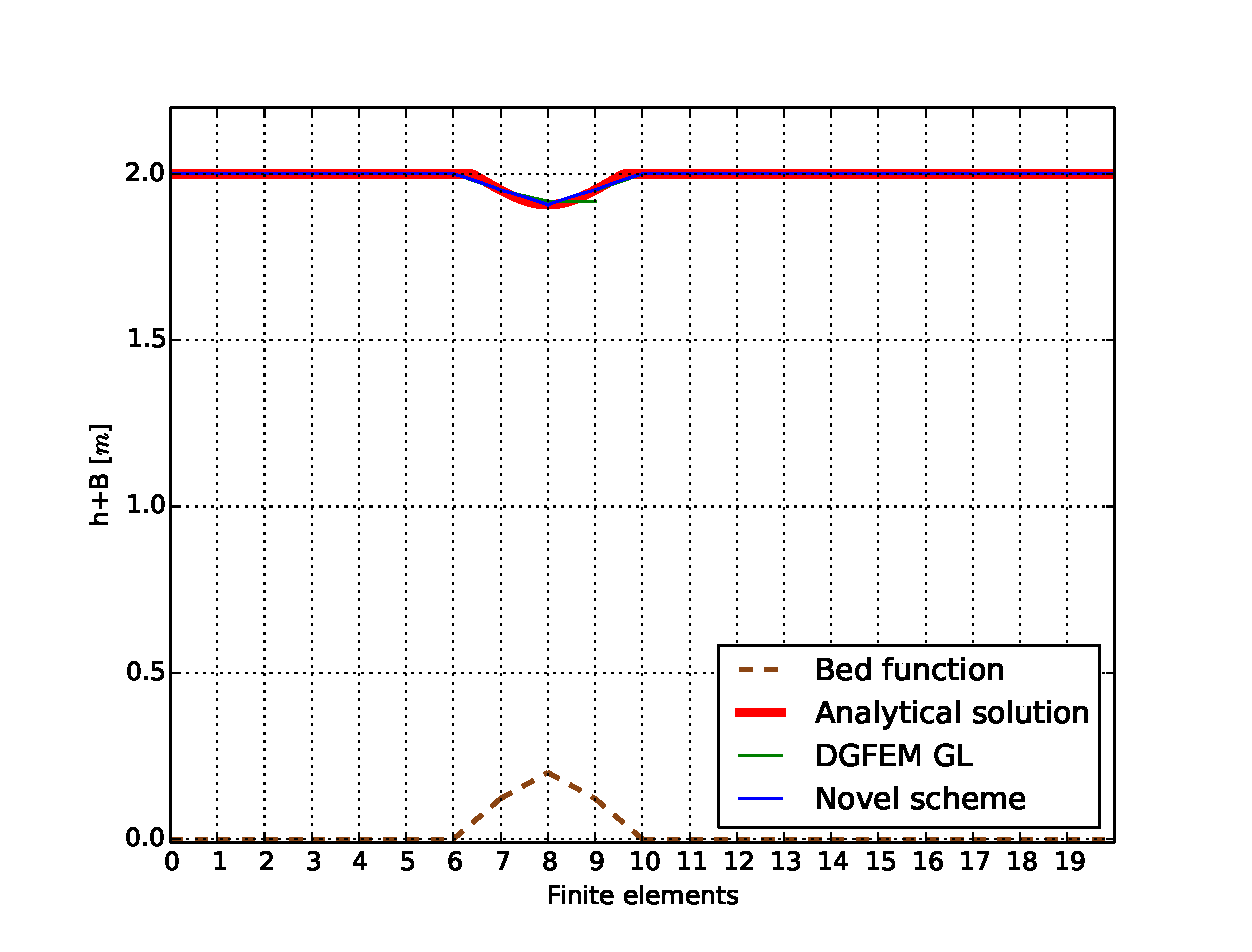
\includegraphics[width=1.0\textwidth]{OBR/bump/subH.eps}
								    \caption{Water depth: subcritical flow.}
								    \label{subH}
								    \end{center}
								\end{minipage}\hspace{15mm}
								\begin{minipage}[t]{0.44\textwidth}
								    \begin{center}
								    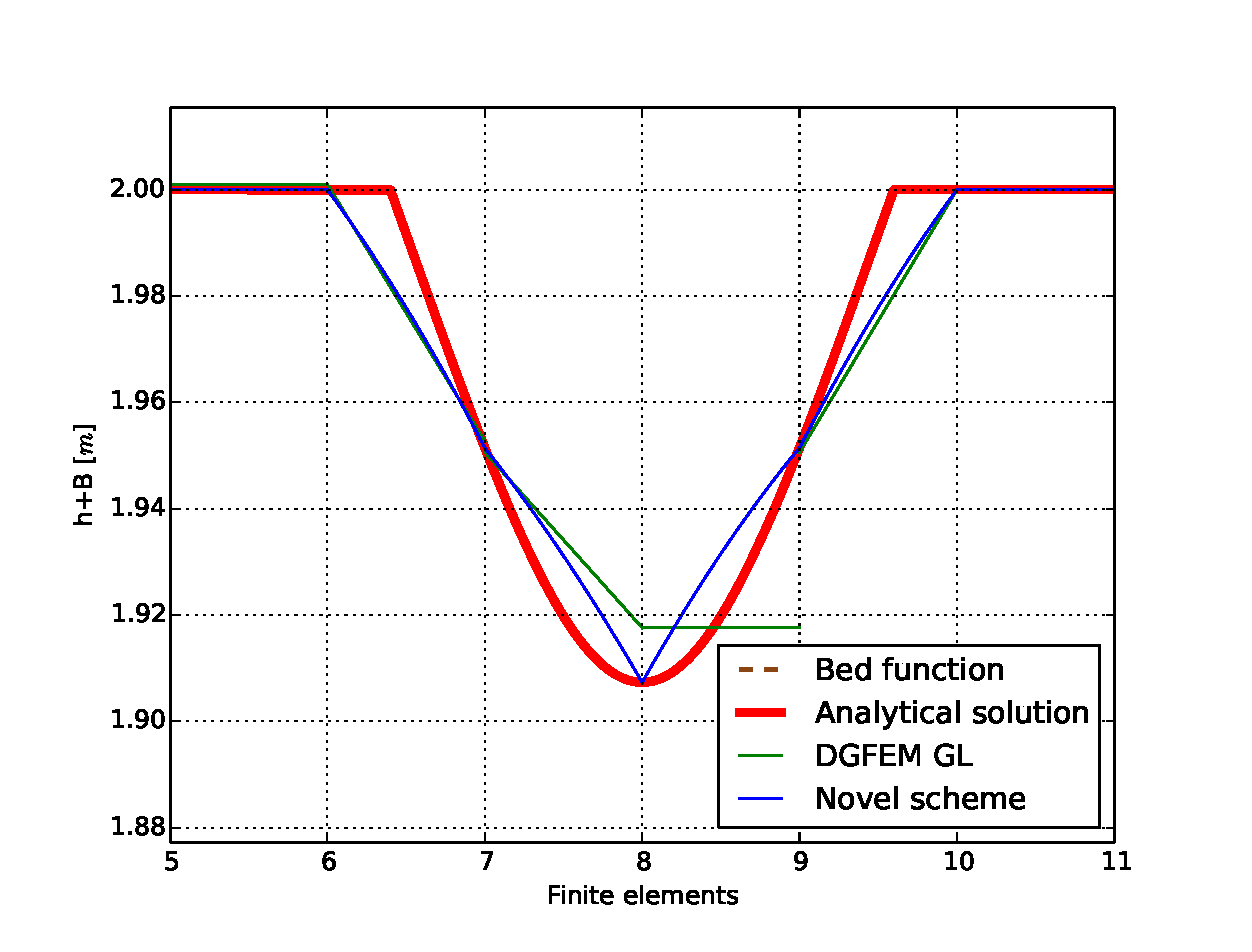
\includegraphics[width=1.0\textwidth]{OBR/bump/subHdet.eps}
								    \caption{Detail of the water depth: subcritical flow.}
								    \label{subHdet}
								    \end{center}
								\end{minipage}
				\end{figure}
				\begin{figure}[!ht]
								\centering
								 \begin{minipage}[t]{0.44\textwidth}
								    \begin{center}
								    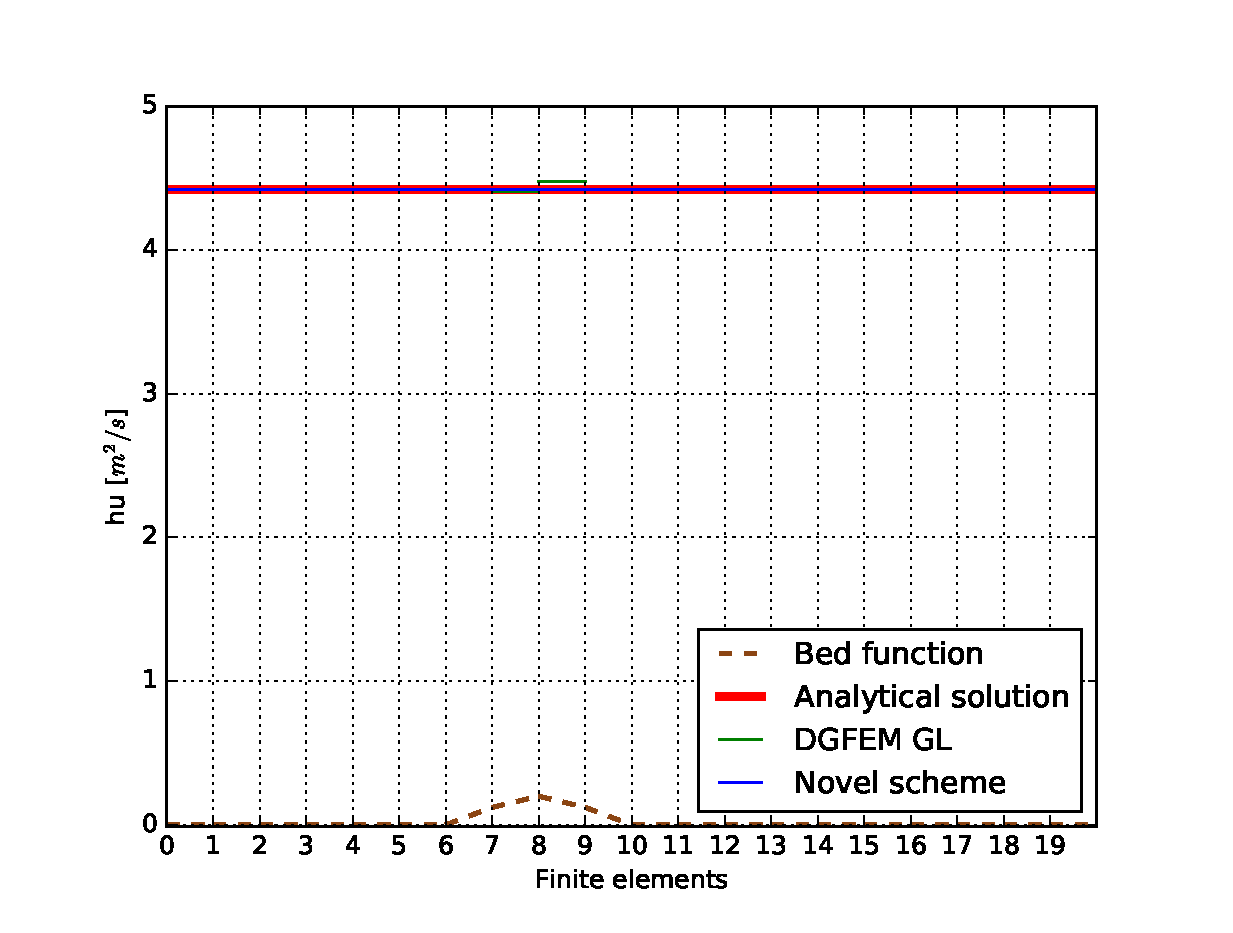
\includegraphics[width=1.0\textwidth]{OBR/bump/subHU.eps}
								    \caption{Discharge: subcritical flow.}
								    \label{subHU}
								    \end{center}
								\end{minipage}\hspace{15mm}
								\begin{minipage}[t]{0.44\textwidth}
								    \begin{center}
								    \includegraphics[width=1.0\textwidth]{OBR/bump/subHUdet.eps}
								    \caption{Detail of the discharge: subcritical flow.}
								    \label{subHUdet}
								    \end{center}
								\end{minipage}
				\end{figure}
The water depth is shown in Figure \ref{subH} and in Figure \ref{subHU} the discharge is shown. Details of the water depth and discharge can be seen in Figures \ref{subHdet} and \ref{subHUdet}. 

The boundary conditions of the transcritical flow without shock are 
\begin{equation}
\begin{array}{c}
q_{inlet}=1.53 \ m^2/s,\\
h_{outlet}=0.66 \ m
\end{array}
\end{equation}
and the analytical solution is given by the resolution of
\begin{equation}
h^3(x)+\left( B(x)-\frac{\text{q} _{inlet}^2}{2g \text{h}_M^2}-h_M-B_M \right) h^2(x)+\frac{\text{q} ^2_{inlet}}{2 g}=0, \quad \forall x \in [0,L]
\end{equation}
where $B_M=\text{max}_{x\in [0,L]}B(x)$ and $\text{h}_M$ is the corresponding water depth.
				\begin{figure}[!ht]
								\centering
								 \begin{minipage}[t]{0.44\textwidth}
								    \begin{center}
								    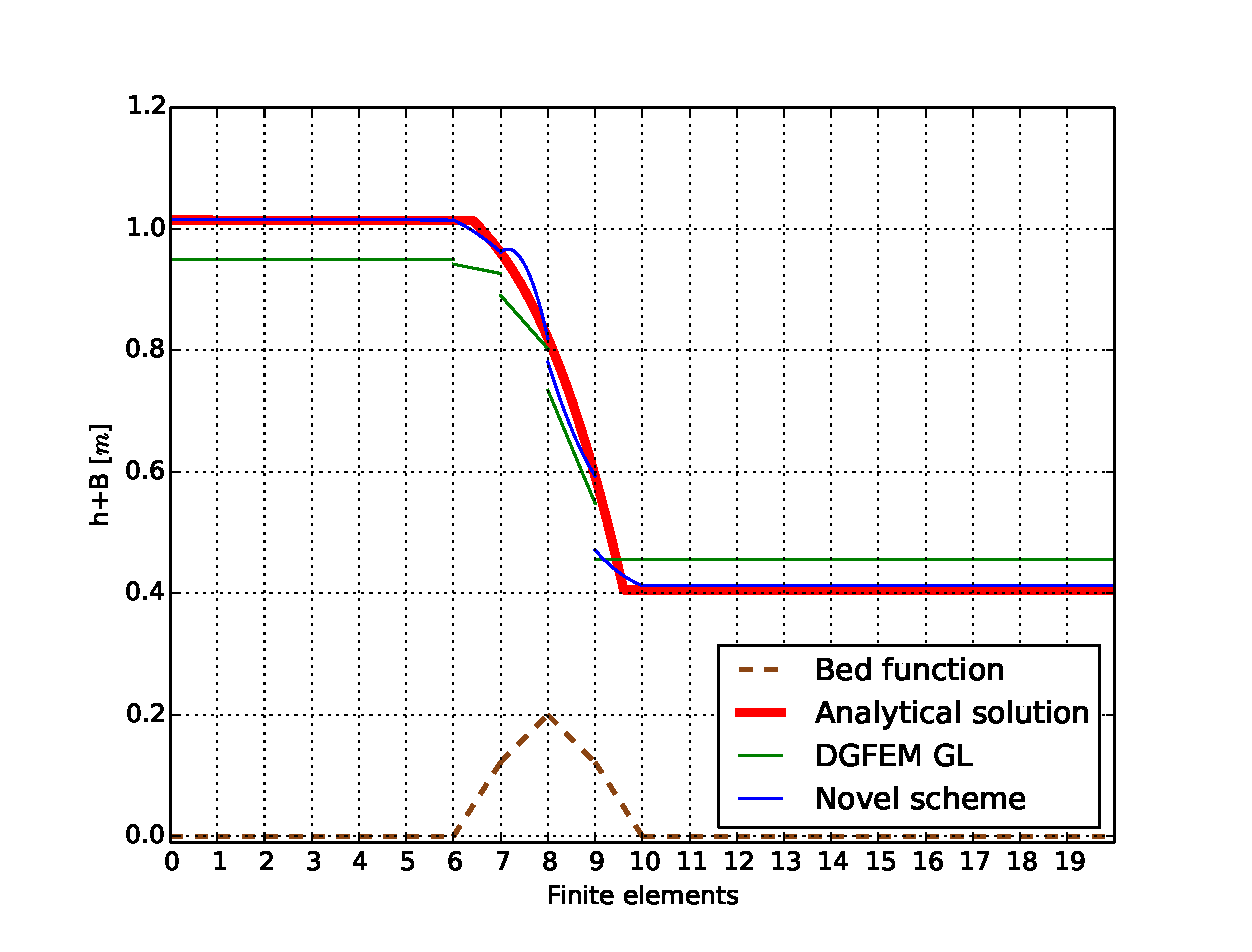
\includegraphics[width=1.0\textwidth]{OBR/bump/transH.eps}
								    \caption{Water depth: transcritical flow without the shock.}
								    \label{transH}
								    \end{center}
								\end{minipage}\hspace{15mm}
								\begin{minipage}[t]{0.44\textwidth}
								    \begin{center}
								    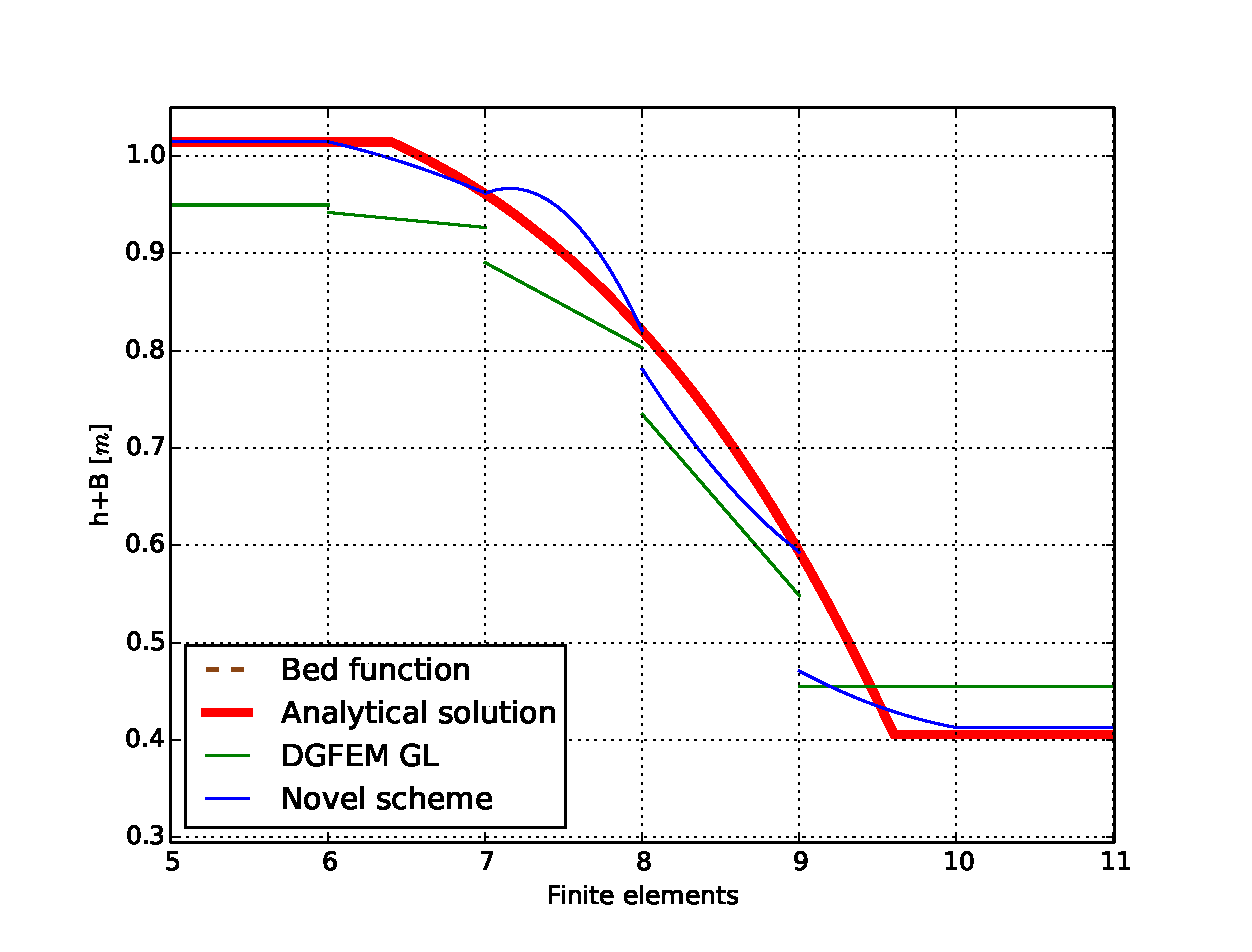
\includegraphics[width=1.0\textwidth]{OBR/bump/transHdet.eps}
								    \caption{Detail of the water depth: transcritical flow without the shock.}
								    \label{transHdet}
								    \end{center}
								\end{minipage}
				\end{figure}
								\begin{figure}[!ht]
								\centering
								 \begin{minipage}[t]{0.44\textwidth}
								    \begin{center}
								    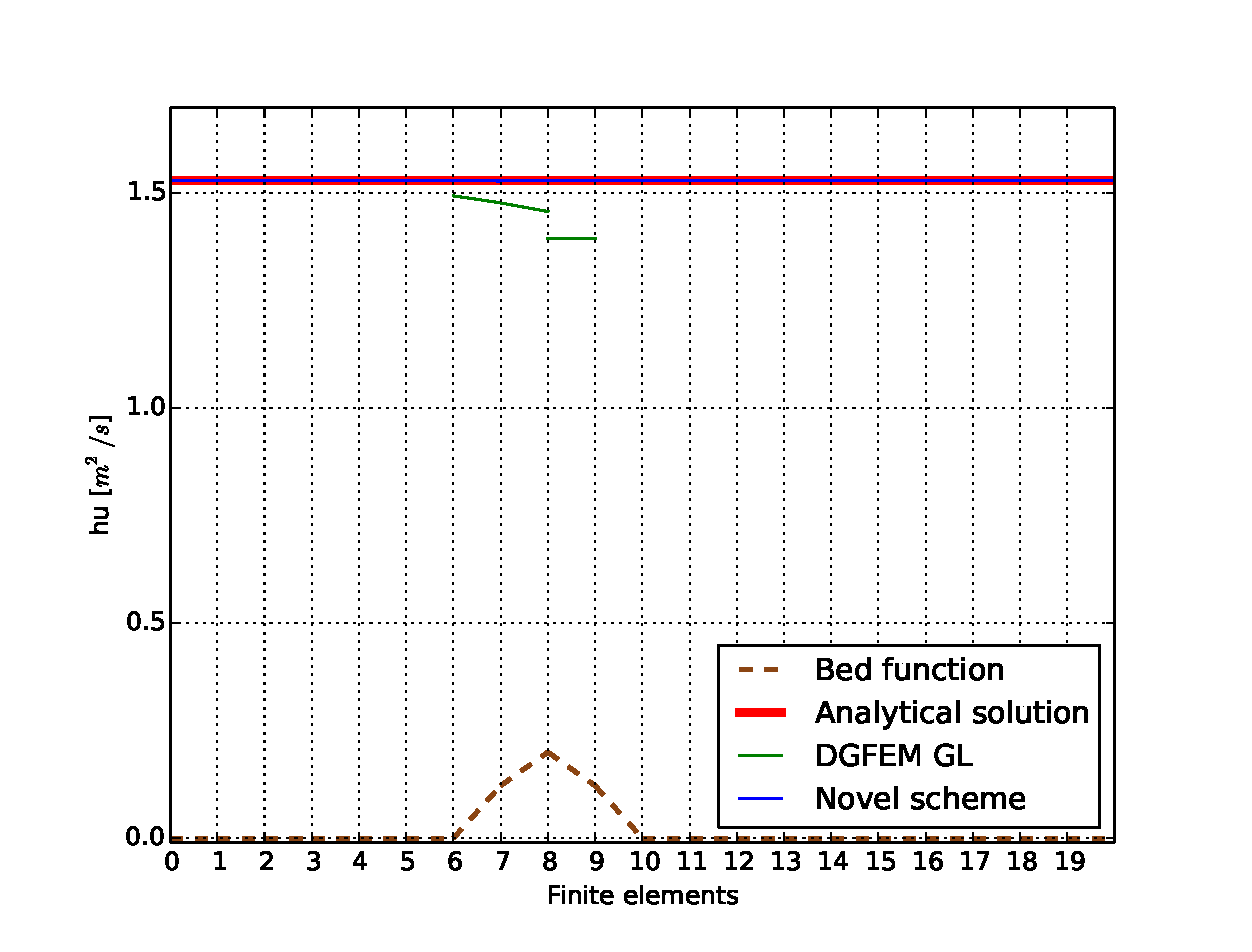
\includegraphics[width=1.0\textwidth]{OBR/bump/transHU.eps}
								    \caption{Discharge: transcritical flow without the shock.}
								    \label{transHU}
								    \end{center}
								\end{minipage}\hspace{15mm}
								\begin{minipage}[t]{0.44\textwidth}
								    \begin{center}
								    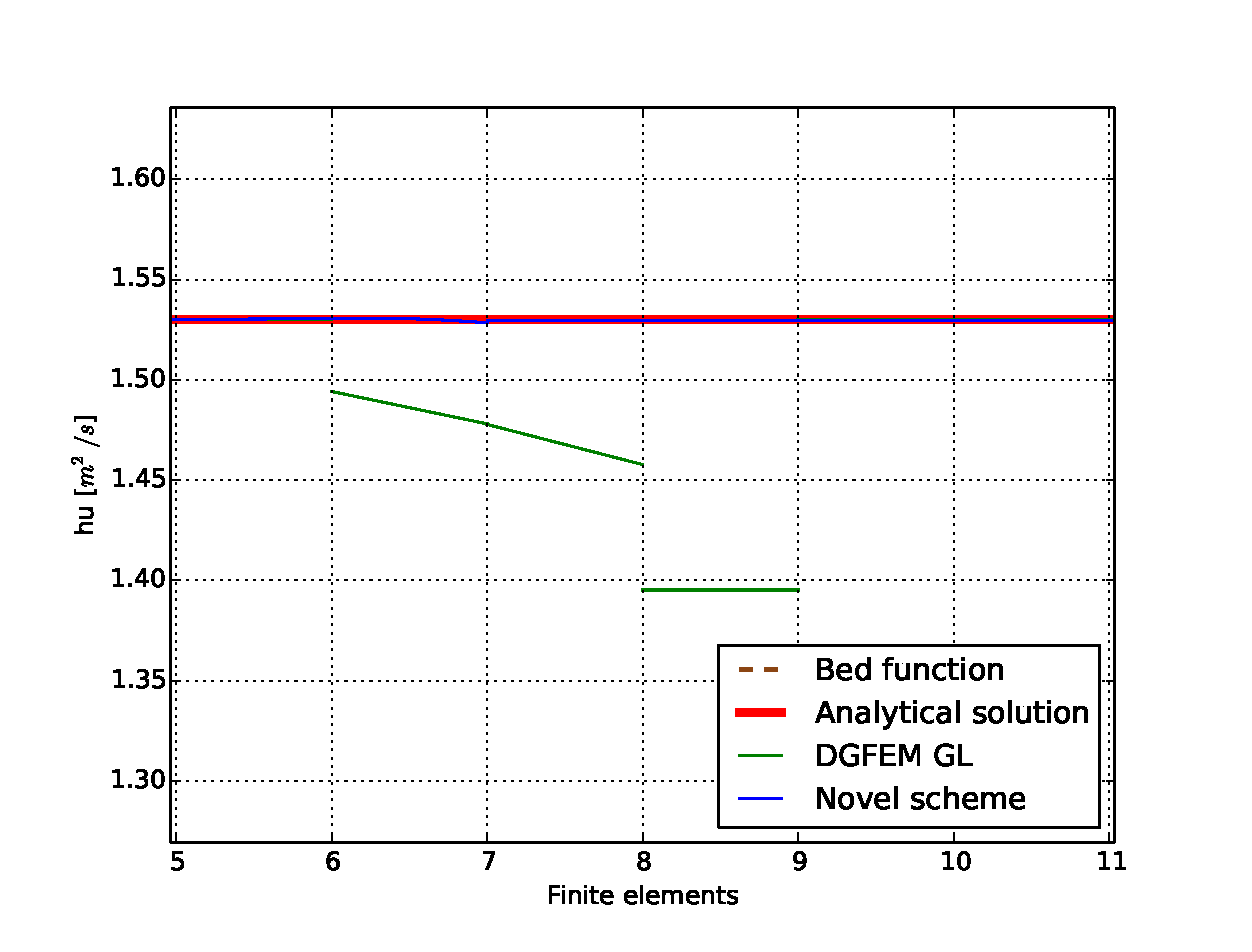
\includegraphics[width=1.0\textwidth]{OBR/bump/transHUdet.eps}
								    \caption{Detail of the discharge: transcritical flow without the shock.}
								    \label{transHUdet}
								    \end{center}
								\end{minipage}
				\end{figure}
In Figures \ref{transH} and \ref{transHdet} the water depth can be seen and the discharge can be seen in Figures \ref{transHU} and \ref{transHUdet}.

Boundary conditions of the transcritical flow with shock are given by 
\begin{equation}
\begin{array}{c}
q_{inlet}=0.18 \ m^2/s,\\
h_{outlet}=0.33 \ m.
\end{array}
\end{equation}
and the analytical solution is given by the resolution of
\begin{equation}\label{desitkaSwa}
\begin{array}{r}
h^3(x _{shock})+\left( B(x _{shock})-\frac{\text{q} ^2_{inlet} }{2g \text{h}^2_M}-\text{h}_M-B_M \right)h^2(x_{shock})+\frac{\text{q} ^2_{inlet}}{2g}=0,\\

h^3(x _{shock})+\left( B(x _{shock})-\frac{\text{q} ^2_{inlet} }{2g \text{h}^2_{outlet}}-\text{h}_{outlet} \right)h^2(x_{shock})+\frac{\text{q} ^2_{inlet}}{2g}=0,\\
\text{q} ^2_{inlet}\left(\frac{1}{h_1}-\frac{1}{h_2}\right)+\frac{g}{2}(h_1^2-h_2^2)=0
\end{array}
\end{equation}
where $h_1$ and $h_2$ are the water depths upstream and downstream respectively. The position of the shock $x_{shock}$ is located thanks to the third relation in system (\ref{desitkaSwa}) which is known as Rankine-Hugoniot’s relation. The reader is referred to \cite{noelle} to see the details.
				\begin{figure}[!ht]
								\centering
								 \begin{minipage}[t]{0.44\textwidth}
								    \begin{center}
								    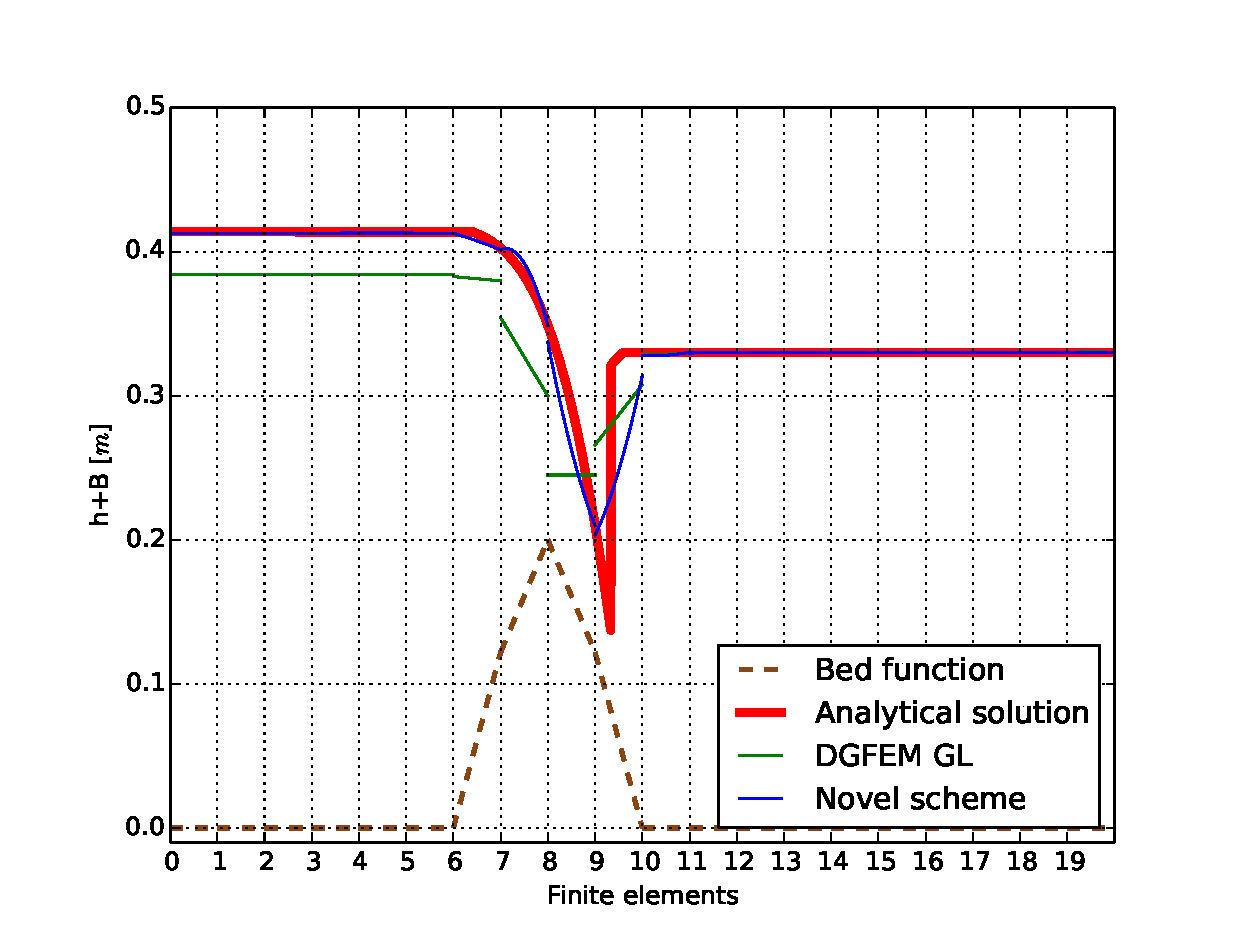
\includegraphics[width=1.0\textwidth]{OBR/bump/shockH.eps}
								    \caption{Water depth: transcritical flow with the shock.}
								    \label{shockH}
								    \end{center}
								\end{minipage}\hspace{15mm}
								\begin{minipage}[t]{0.44\textwidth}
								    \begin{center}
								    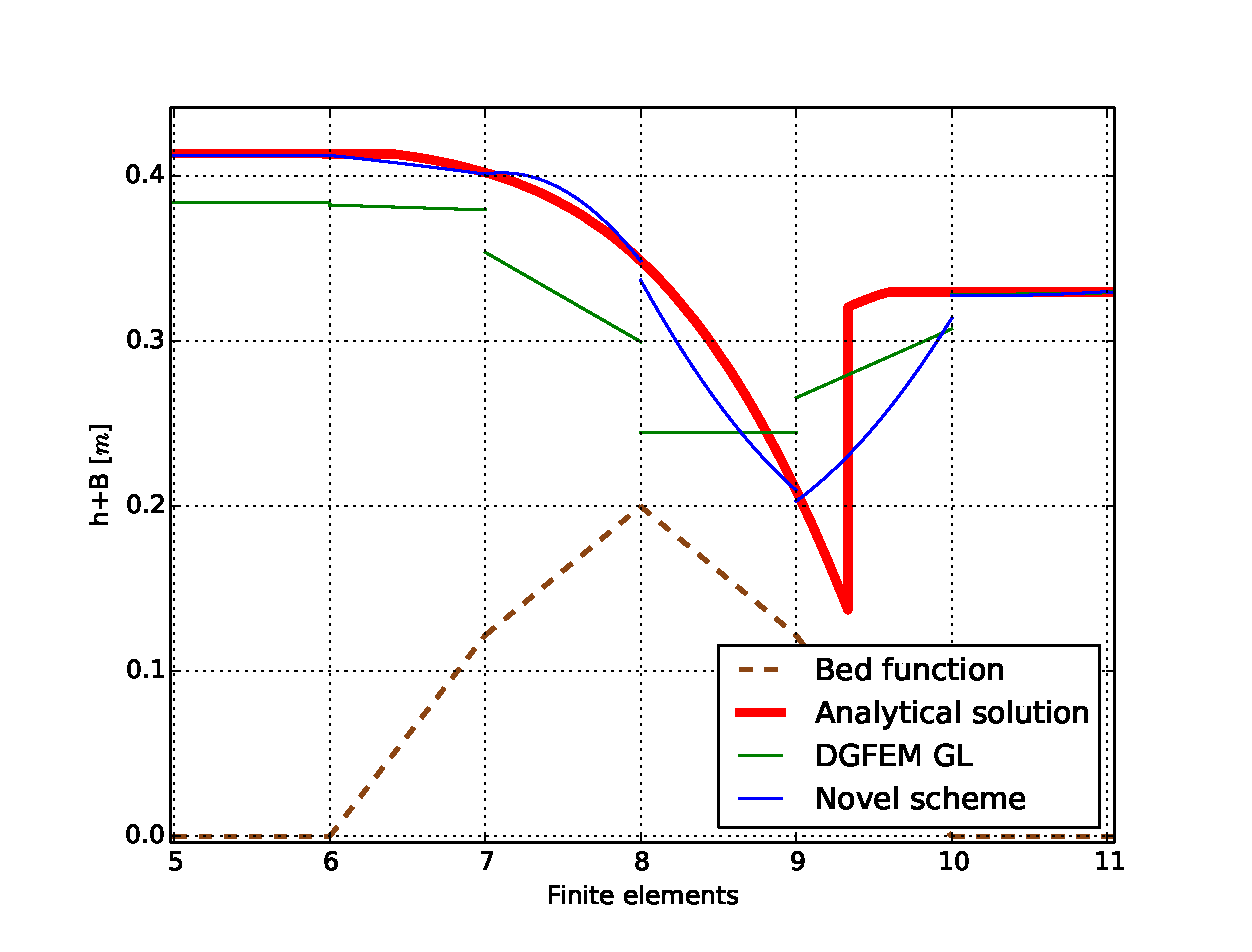
\includegraphics[width=1.0\textwidth]{OBR/bump/shockHdet.eps}
								    \caption{Detail of the water depth: transcritical flow with the shock.}
								    \label{shockHdet}
								    \end{center}
								\end{minipage}
				\end{figure}
								\begin{figure}[!ht]
								\centering
								 \begin{minipage}[t]{0.44\textwidth}
								    \begin{center}
								    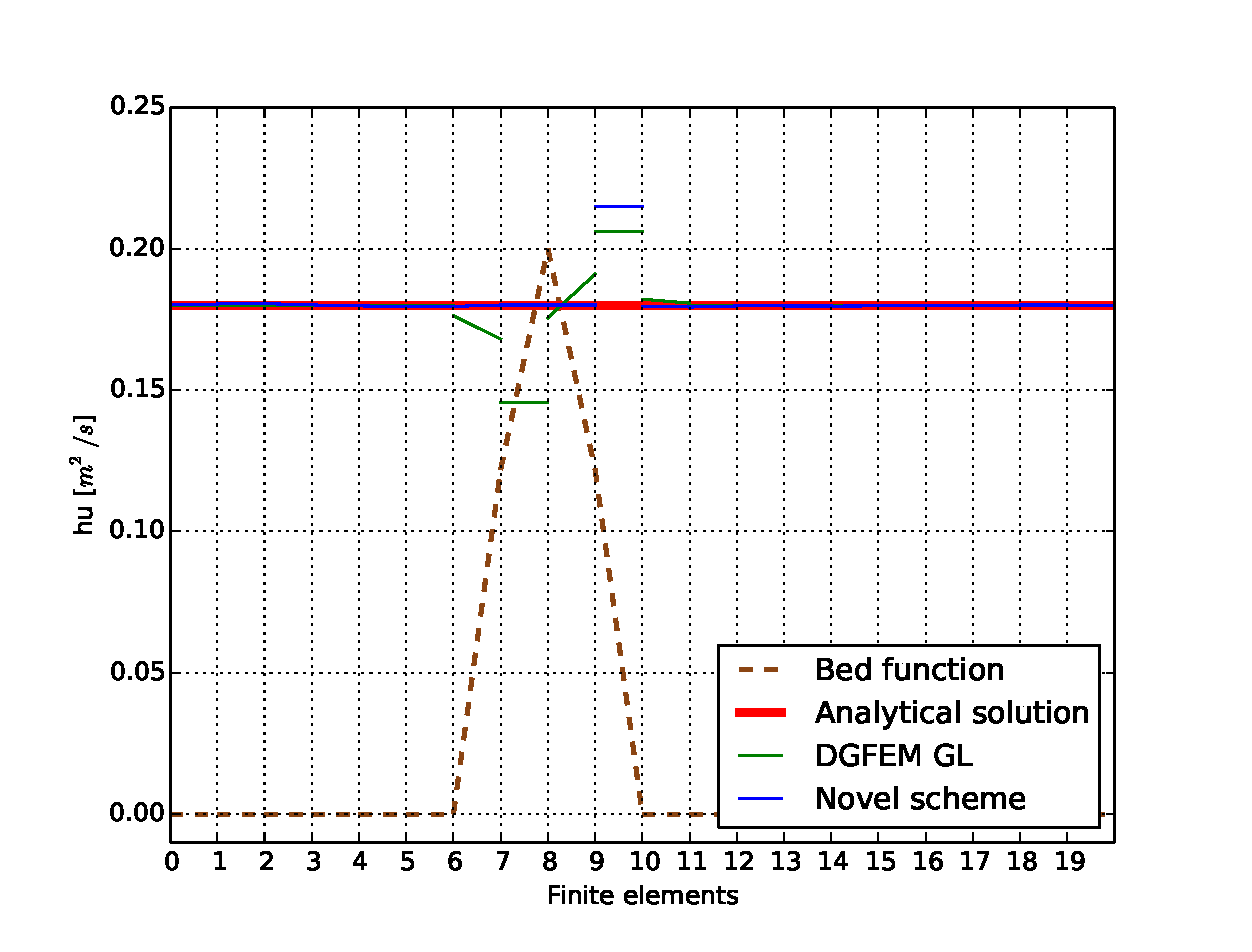
\includegraphics[width=1.0\textwidth]{OBR/bump/shockHU.eps}
								    \caption{Discharge: transcritical flow with the shock.}
								    \label{shockHU}
								    \end{center}
								\end{minipage}\hspace{15mm}
								\begin{minipage}[t]{0.44\textwidth}
								    \begin{center}
								    \includegraphics[width=1.0\textwidth]{OBR/bump/shockHUdet.eps}
								    \caption{Detail of the discharge: transcritical flow with the shock.}
								    \label{shockHUdet}
								    \end{center}
								\end{minipage}
				\end{figure}
Numerical solution of the water depth is shown in Figures \ref{shockH} and \ref{shockHdet}. In Figures \ref{shockHU} and \ref{shockHUdet} the discharge is shown.